\documentclass{article} % Defines the document class, article is commonly used
\usepackage[shortlabels]{enumitem}
\usepackage{amsmath}    % Allows for more advanced math formatting
\usepackage{amssymb}    % Provides additional mathematical symbols
\usepackage{amsthm}     % \qed
\usepackage{graphicx}   % image
\usepackage{float}      % image placement
\usepackage{siunitx}
\usepackage{hyperref}
\hypersetup{
    colorlinks=true,       % false: boxed links; true: colored links
    linkcolor=black,       % color of internal links
}
\usepackage[margin=1.5in]{geometry}

\begin{document}

\title{EEC133 Lab 2: Loop Antennas}
\author{Josias Moreno Ixta, Michael Chen, Tao Wang, Xaviera Azodoh}
\date{\today}

\maketitle
\tableofcontents

\section*{Pre-Lab}
\addcontentsline{toc}{section}{Pre-Lab}

\subsection*{Part 1: Loop Antenna Design}
\addcontentsline{toc}{subsection}{Part 1: Loop Antenna Design}

\subsubsection*{Questions:}
\begin{enumerate}[]
    \item $r = 0.0064 \si{m}$. $\lambda = \frac{c}{f} = 0.12 \si{m}$. $r \leq \frac{\lambda}{6 \pi} \approx 0.00637 \si{m}$.
    \item
          \[\text{Radiation Resistance: }320 \pi^6 \left(\frac{0.00637}{0.12}\right)^4 = 2.44 \Omega \]
          \[\text{Directivity: } 1.5\]
          \[\text{Half-power beamwidth: } \frac{\pi}{2}\]
          \[\text{Far Field Requirement: } r >> \frac{0.12}{2\pi} = 0.019 \si{m}\]
    \item $C = 2.34 \text{ fF}$. Since $R_A = 18.32 \Omega$, $X_A = 705.38 \Omega$, and $\omega = 2 \pi \times 2.5 \times 10^9$, $C = \frac{R_{A}}{\omega (R_{A}^{2}+X_{A}^{2})} = 2.34 \text{ fF}$
    \item
          \begin{enumerate}[(a)]
              \item Screenshot of HFSS Model
                    \begin{figure}[H]
                        \centering
                        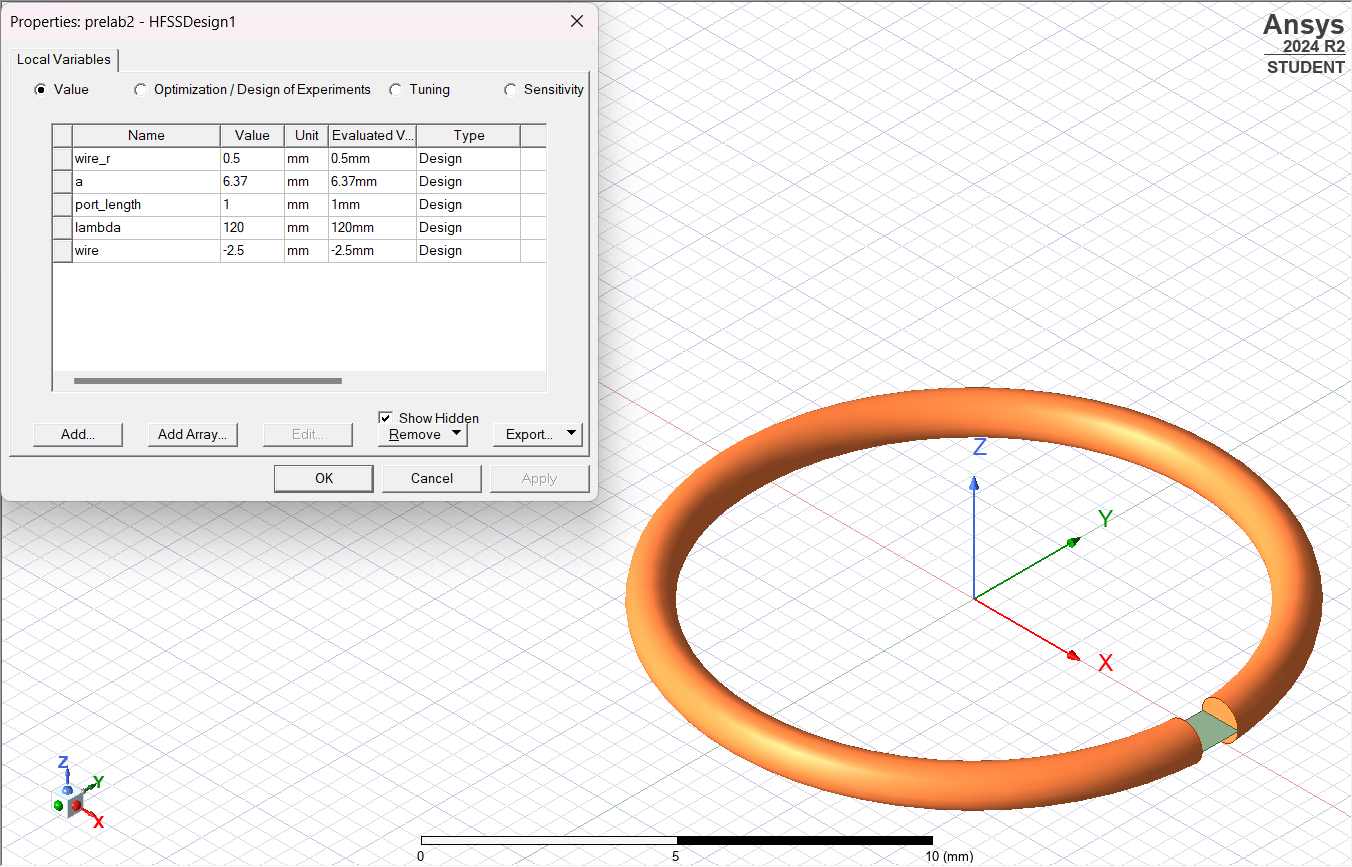
\includegraphics[width=0.5\textwidth]{./image/figure1.png}
                        \caption{HFSS Loop Antenna Model}
                    \end{figure}
              \item The return loss plot shows the $20 \log |\Gamma| $, the reflection coefficient of the antenna, across different frequencies.
                    \begin{figure}[H]
                        \centering
                        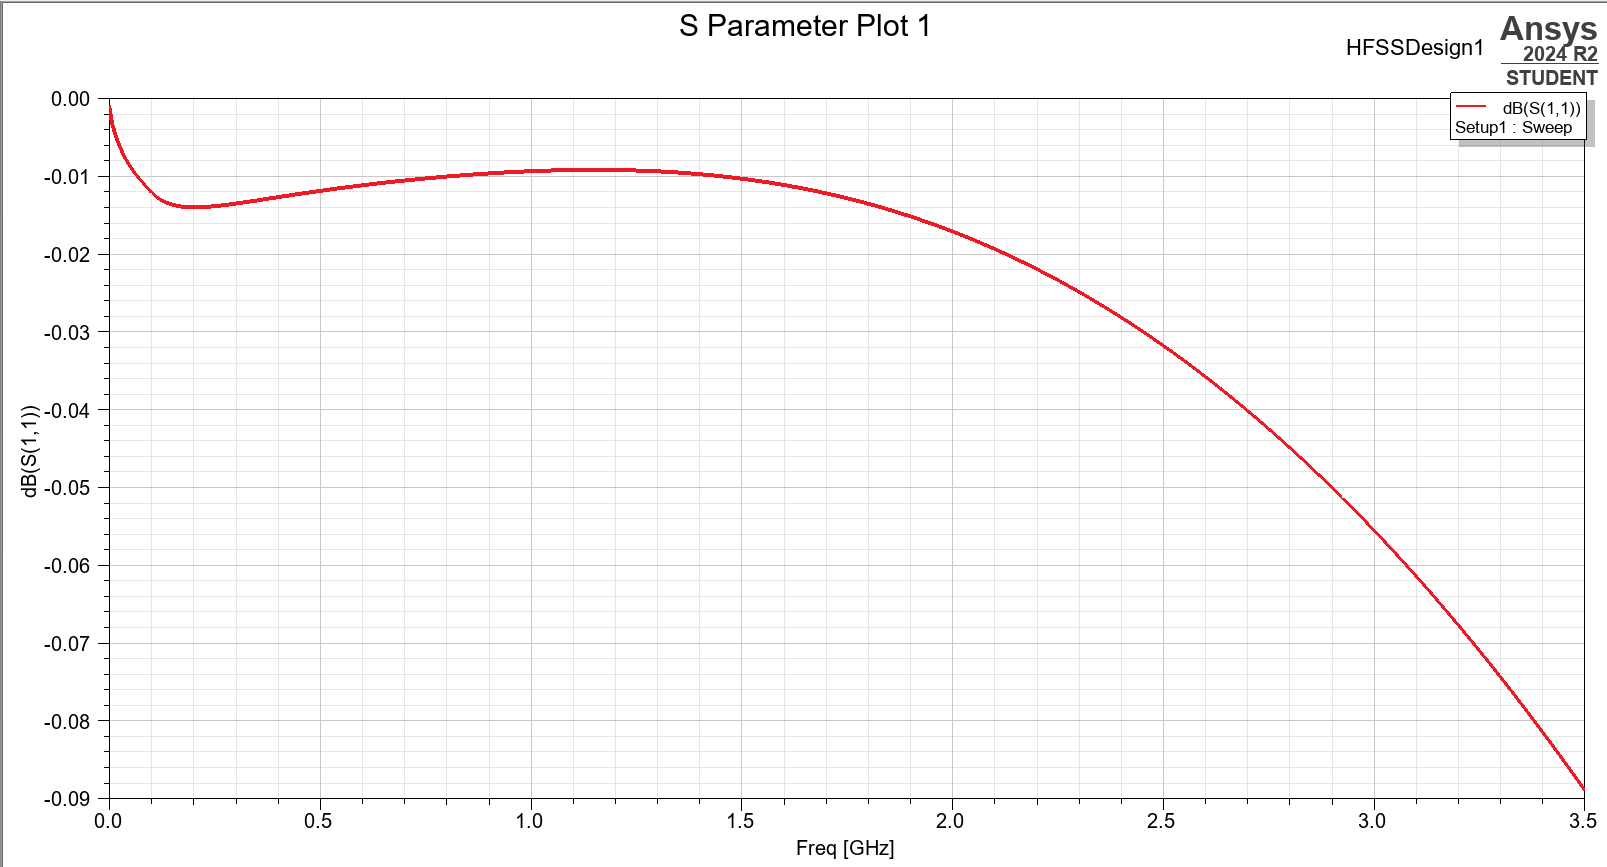
\includegraphics[width=0.5\textwidth]{./image/figure2.png}
                        \caption{$S_{1,1}$ Parameter}
                    \end{figure}
              \item Plot the 3D directivity pattern at 2.5 GHz.
                    \begin{figure}[H]
                        \centering
                        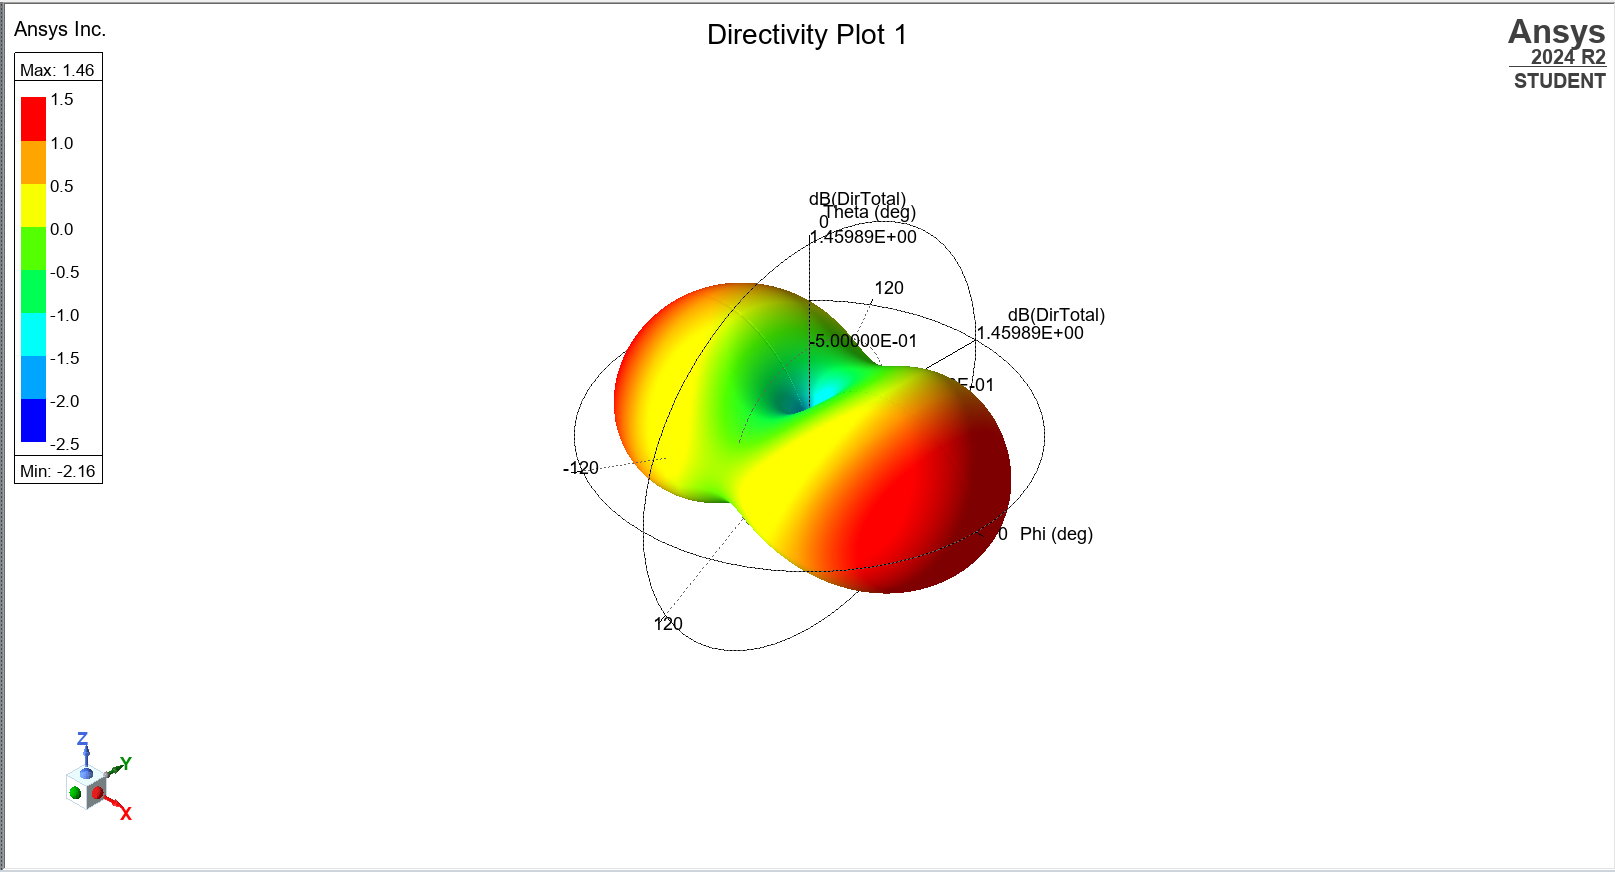
\includegraphics[width=0.5\textwidth]{./image/figure3.png}
                        \caption{3D Directivity Pattern at 2.5 GHz}
                    \end{figure}
              \item Plot the directivity pattern with $\phi = 90 ^{\circ}$ and $0^{\circ} \geq \theta \leq 180 ^{\circ}$.
                    \begin{figure}[H]
                        \centering
                        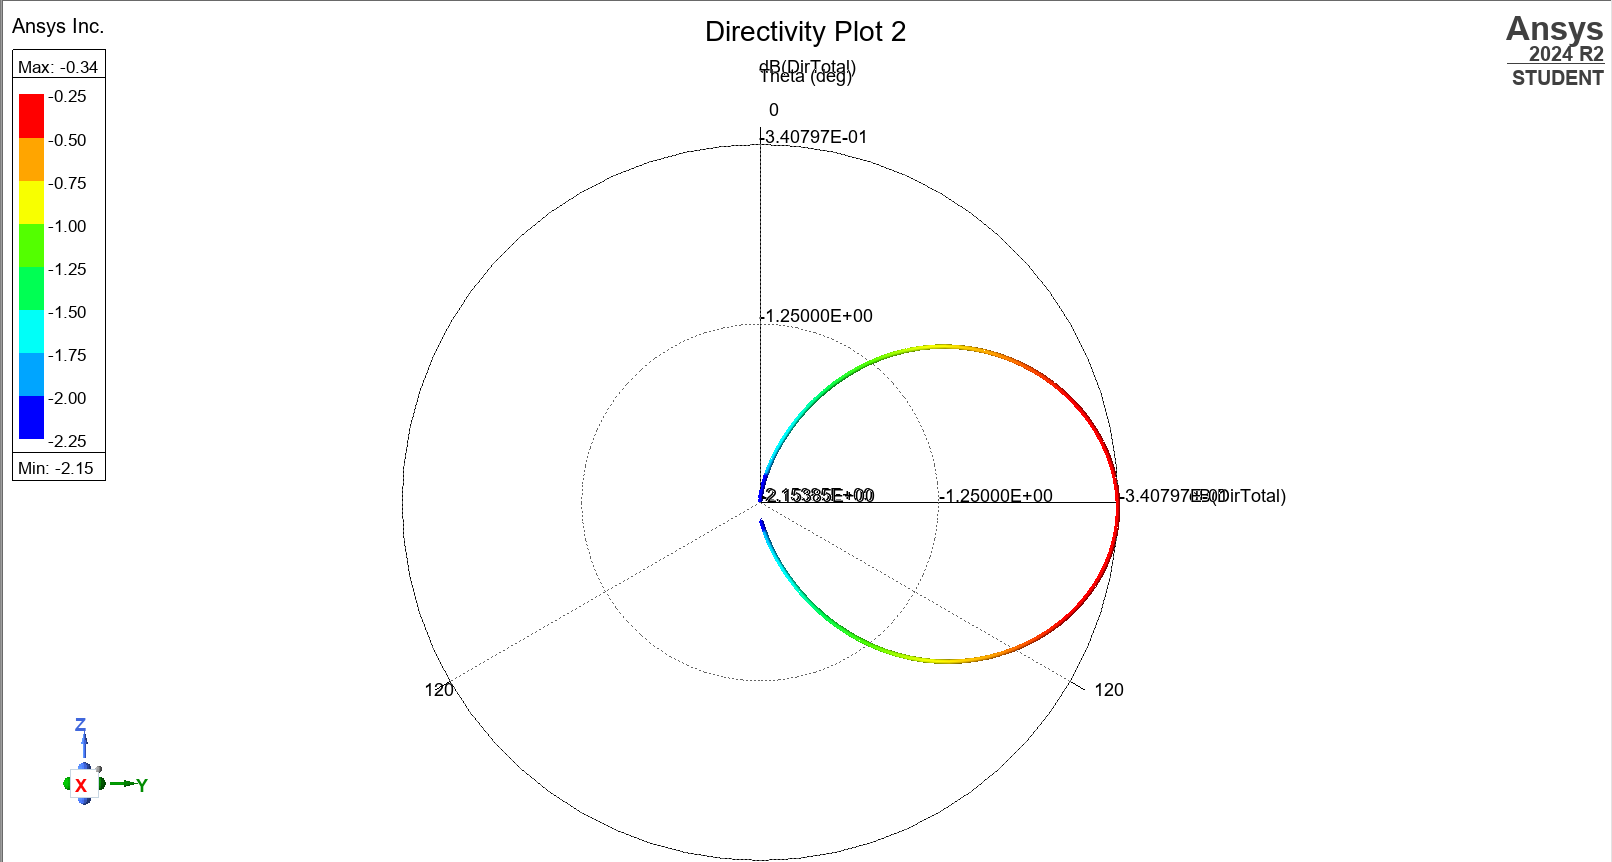
\includegraphics[width=0.5\textwidth]{./image/figure4.png}
                        \caption{Directivity Pattern at $\phi = 90 ^{\circ}$}
                    \end{figure}
              \item The expected input resistance is $2.44 \Omega$, but the simulated resistance is $18.32 \Omega$, so the results are very different. However, the simulated reactance makes sense because it's very large compared to the resistance. Therefore, the reflection coefficient is about -1, which matches the $S_{1, 1}$ plot at 2.5 GHz.
                    \begin{figure}[H]
                        \centering
                        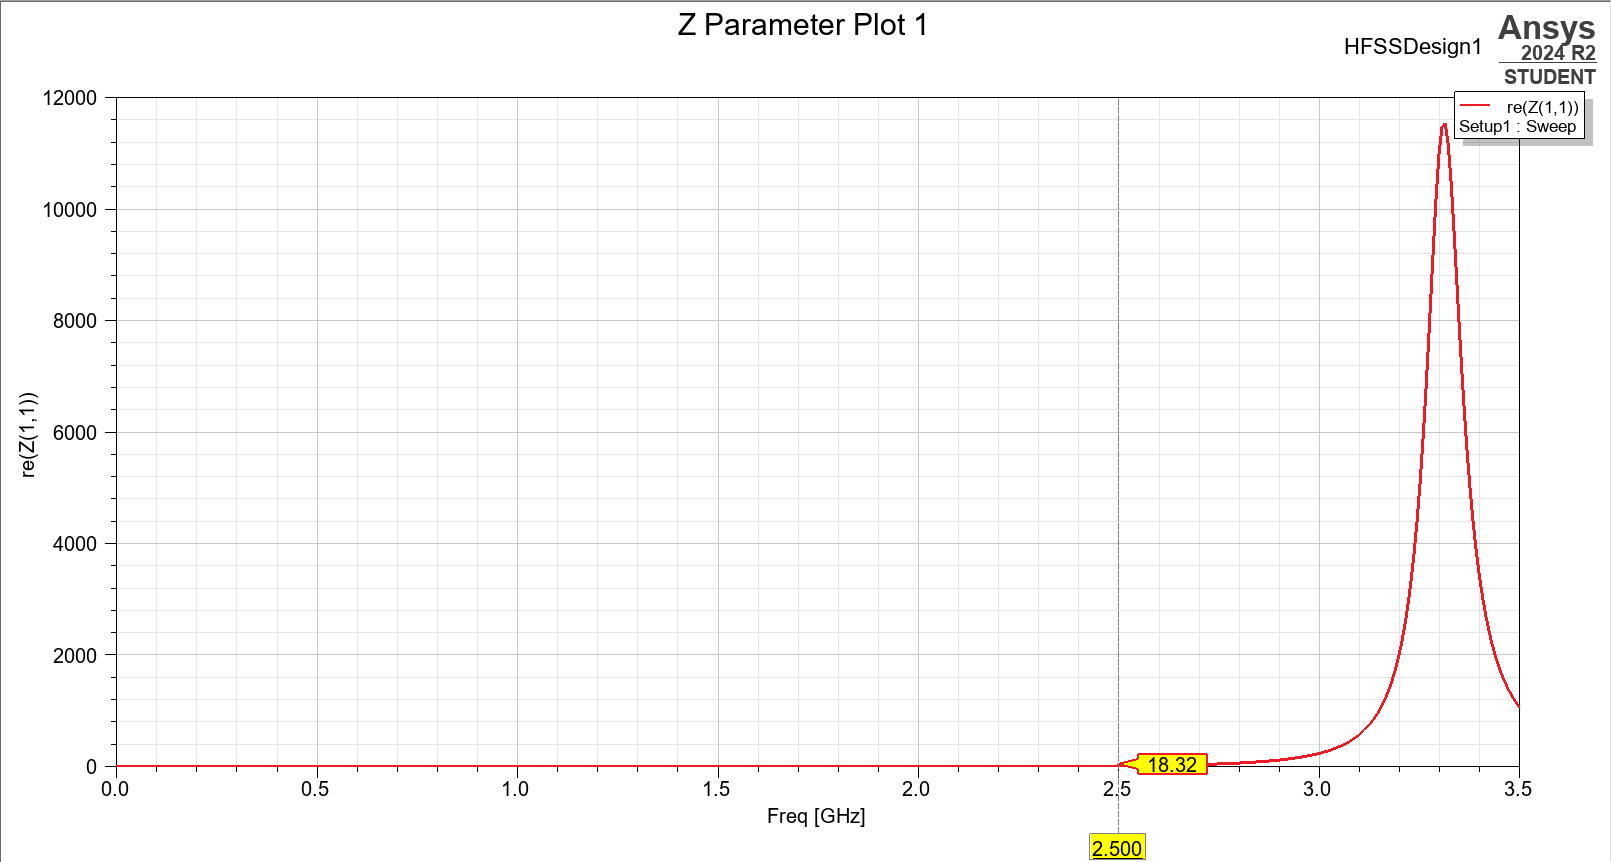
\includegraphics[width=0.5\textwidth]{./image/figure5.png}
                        \caption{Re$(Z_{1, 1}$) at 2.5 GHz}
                    \end{figure}
                    \begin{figure}[H]
                        \centering
                        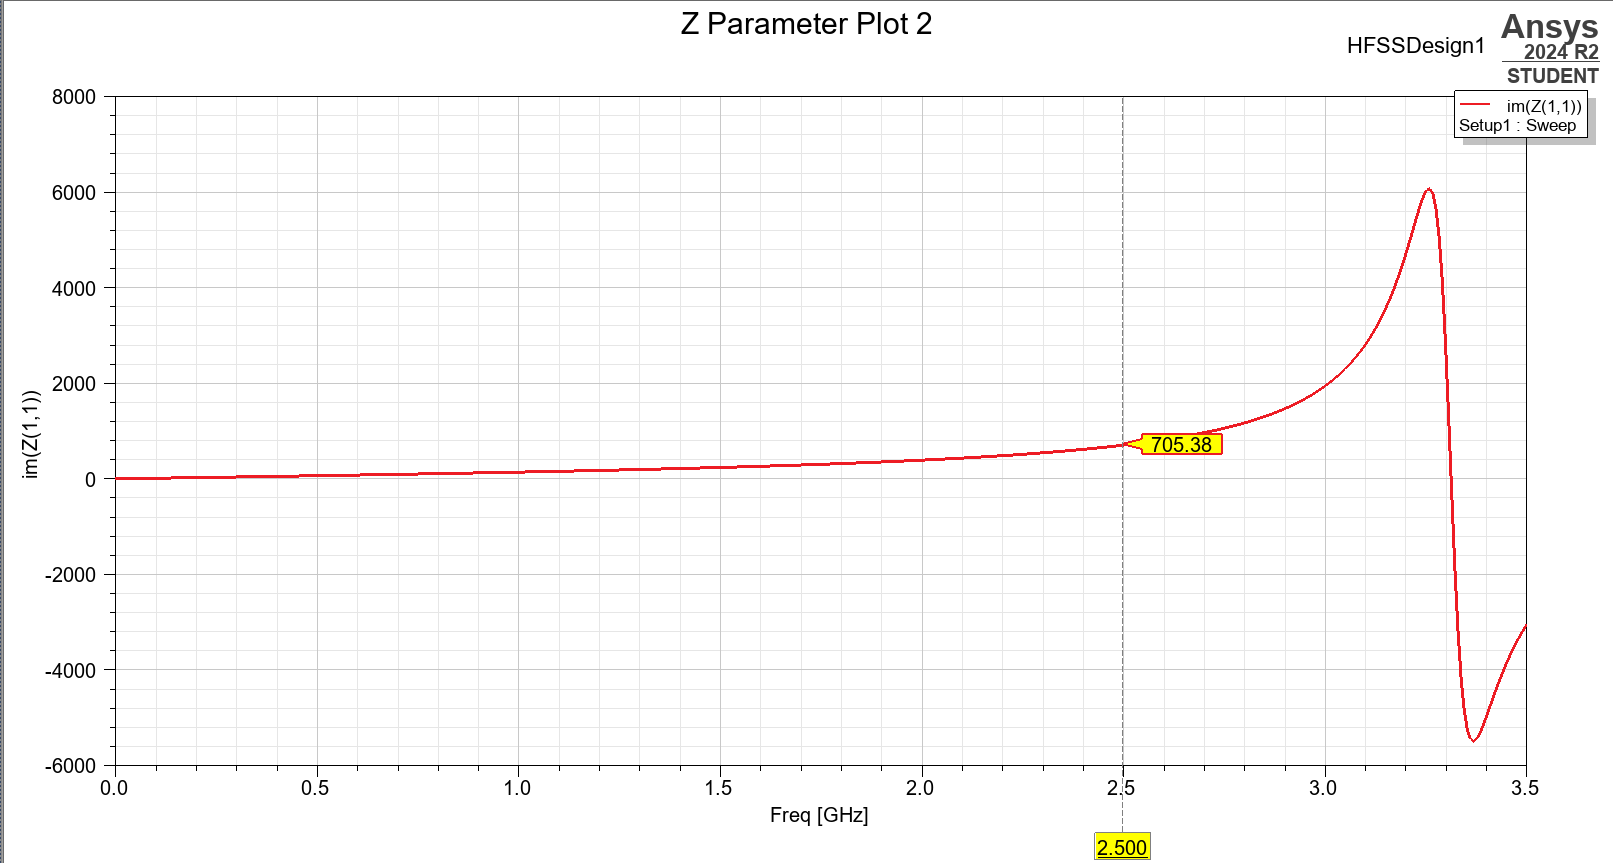
\includegraphics[width=0.5\textwidth]{./image/figure6.png}
                        \caption{Im$(Z_{1, 1}$) at 2.5 GHz}
                    \end{figure}
              \item To find the radiation efficiency, we'll plot the gain at 2.5 GHz and use $e = \frac{G_0}{D_0}$
                    Since $G_0 = 1.35$ dB and $D_0 = 1.46$ dB, the efficiency is 92.5\%.
                    \begin{figure}[H]
                        \centering
                        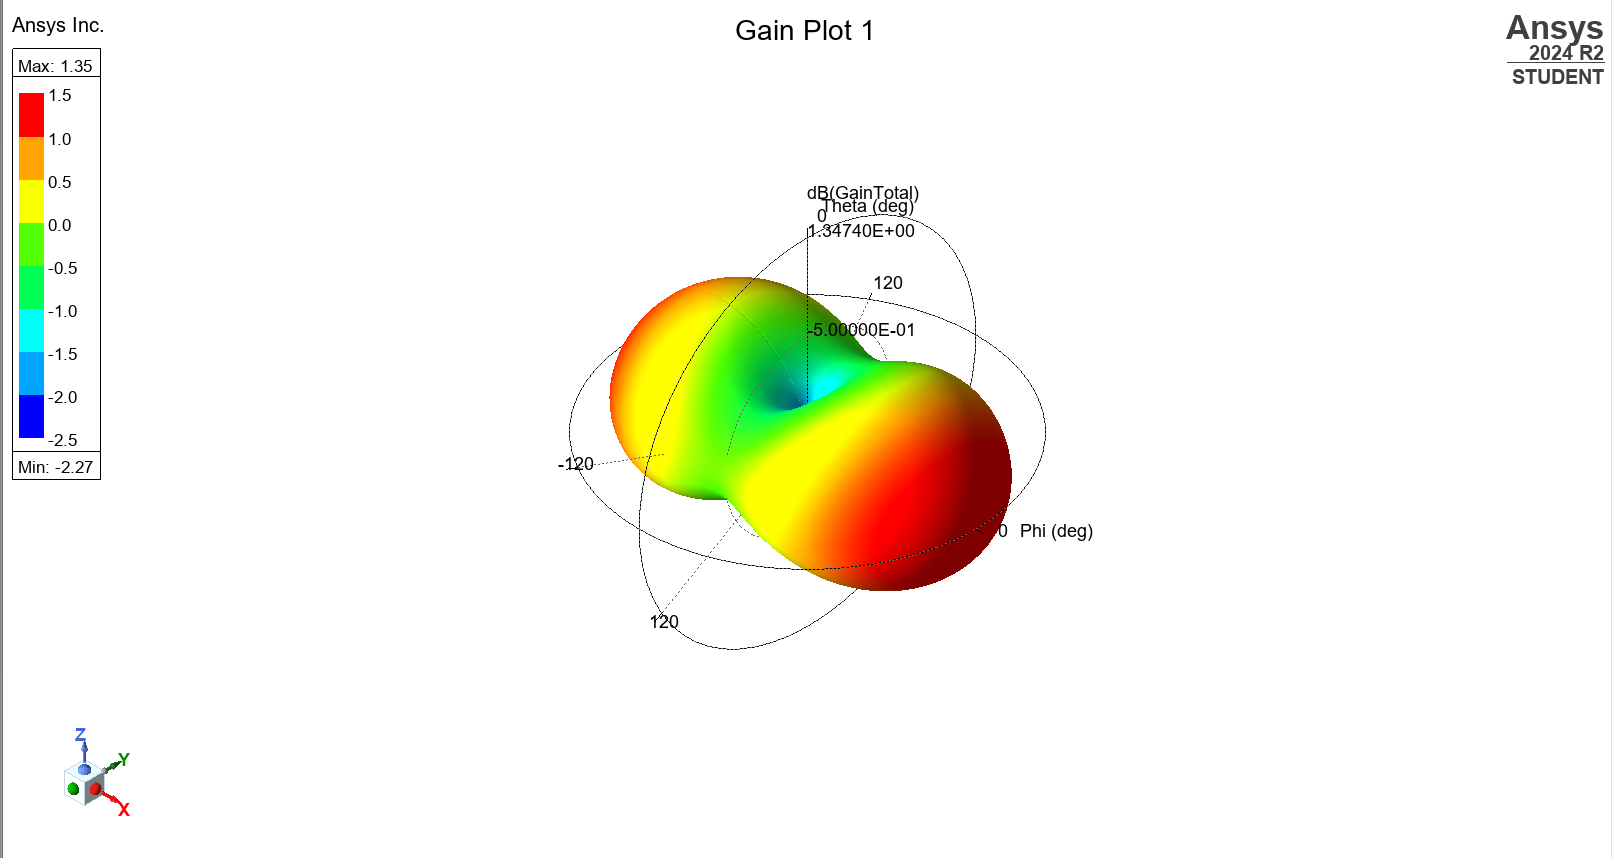
\includegraphics[width=0.5\textwidth]{./image/figure7.png}
                        \caption{Antenna Gain at 2.5 GHz}
                    \end{figure}
              \item The electric field at $z = 10$ mm plane.
                    \begin{figure}[H]
                        \centering
                        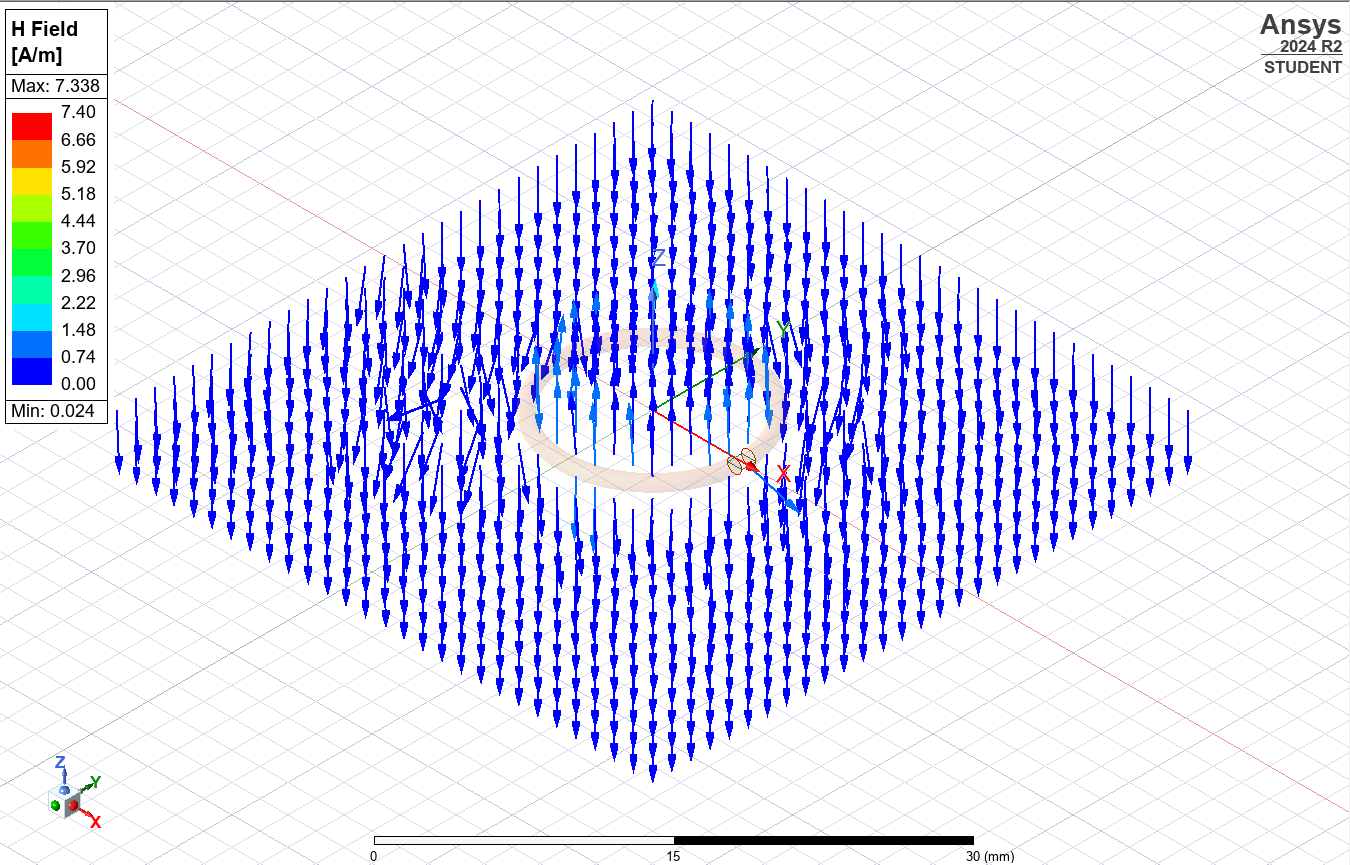
\includegraphics[width=0.5\textwidth]{./image/figure8.png}
                        \caption{Electric Field}
                    \end{figure}
              \item The magnetic field at $z = 10$ mm plane.
                    \begin{figure}[H]
                        \centering
                        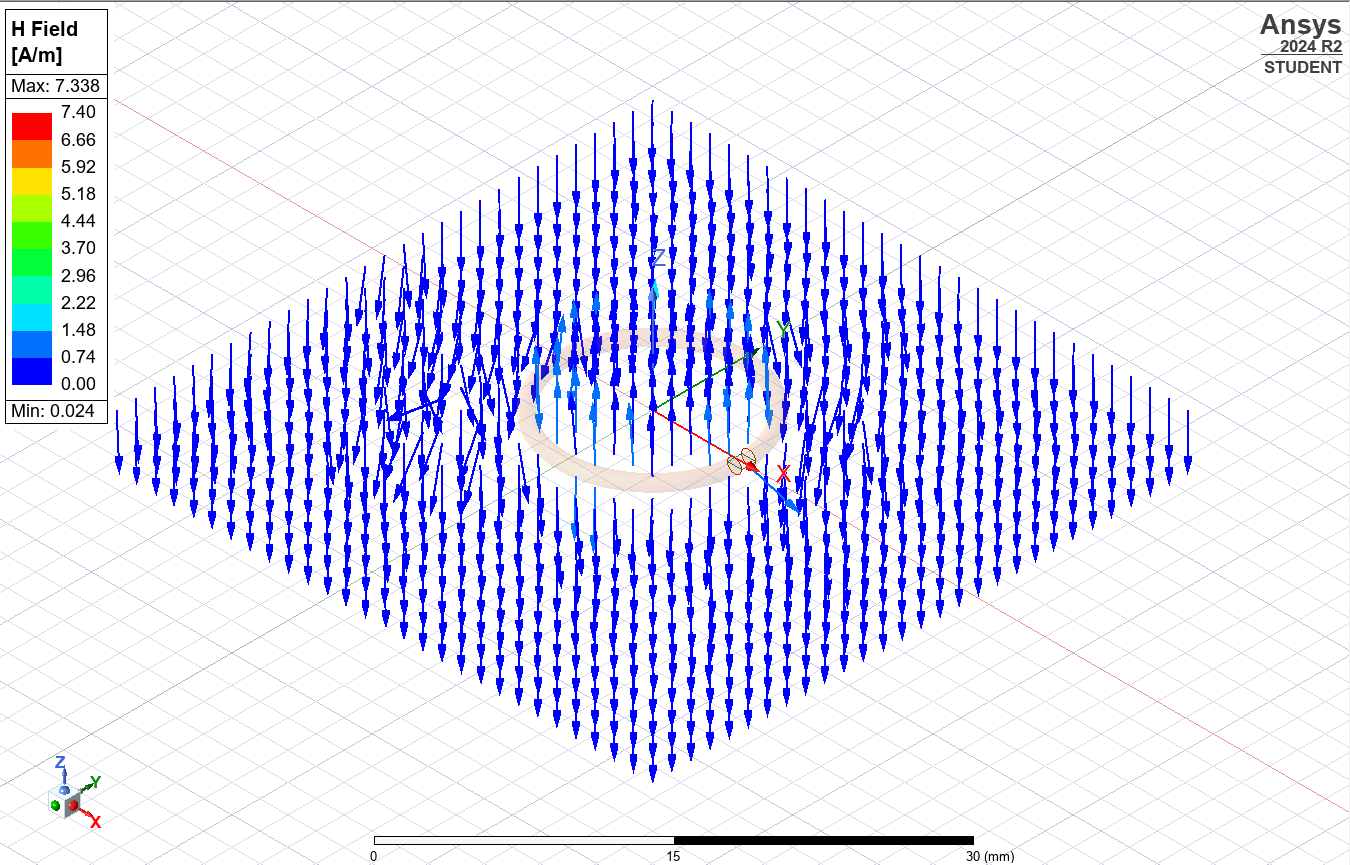
\includegraphics[width=0.5\textwidth]{./image/figure9.png}
                        \caption{Magnetic Field}
                    \end{figure}
              \item The plots make sense because the magnetic field looks like the dipole field.
              \item No. The antenna's input resistance is too small, making the $50\Omega$ transmission line hard to match its impedance.
          \end{enumerate}
\end{enumerate}

\subsection*{Part 2: More Noise Calculations}
\addcontentsline{toc}{subsection}{Part 2: More Noise Calculations}

\subsubsection*{Questions:}
\begin{enumerate}
    \item $R_{in}$ and $R_{out}$ are typically $50 \Omega$ to avoid wave reflection in $R_{in}$ by matching the characteristics impedance in the input and output transmission line. $R_{out}$
    \item Noise =
          \[9.1 \times 10^{-10} \frac{V}{\sqrt{Hz}}\]
          This unit means that the noise voltage is $9.1*10^{-10}$ volts per unit of the frequency bandwidth.
    \item $R_{in} = 0.489 \Omega$, so $\tau = 0.019$. The small transmission coefficient implies that very little power will be transmitted to the amplifier, so the signal amplification will be poor.
\end{enumerate}

\section*{Post-Lab}
\addcontentsline{toc}{section}{Post-Lab}
\subsubsection*{Questions:}
\begin{enumerate}
    \item Total length = 0.3 m. The original length is accurate enough as lab 1 measurements showed.
    \item Resonant frequency at 1.06 GHz. The loop is 0.94 fraction of wavelengths. The result shows that reflection from the antenna is minimized at 1.06 GHz.
          \begin{figure}[H]
              \centering
              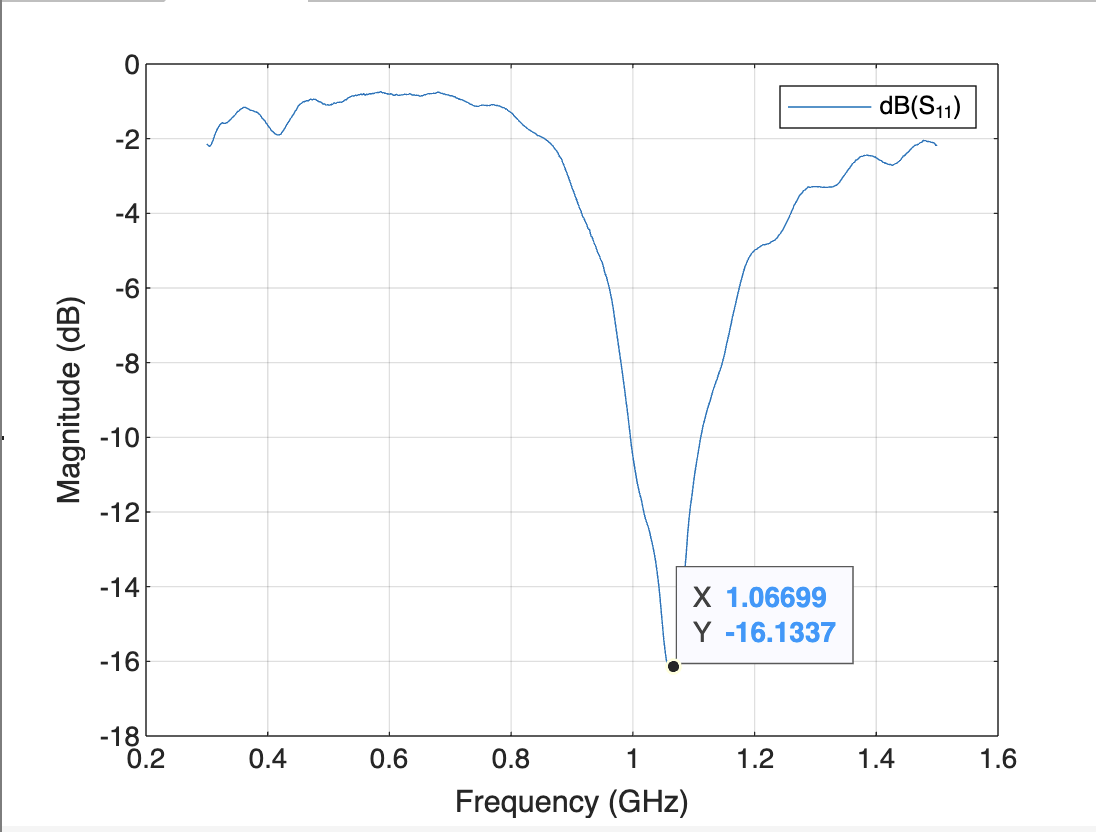
\includegraphics[width=0.5\textwidth]{./image/figure10.png}
              \caption{$S_{1, 1}$ at $90^{\circ}$}
          \end{figure}
    \item The input impedance makes sense because the real and imaginary parts has similar shape to that of the simulated results. However, the scale of the impedance is much smaller than those of the simulation.
          \begin{figure}[H]
              \centering
              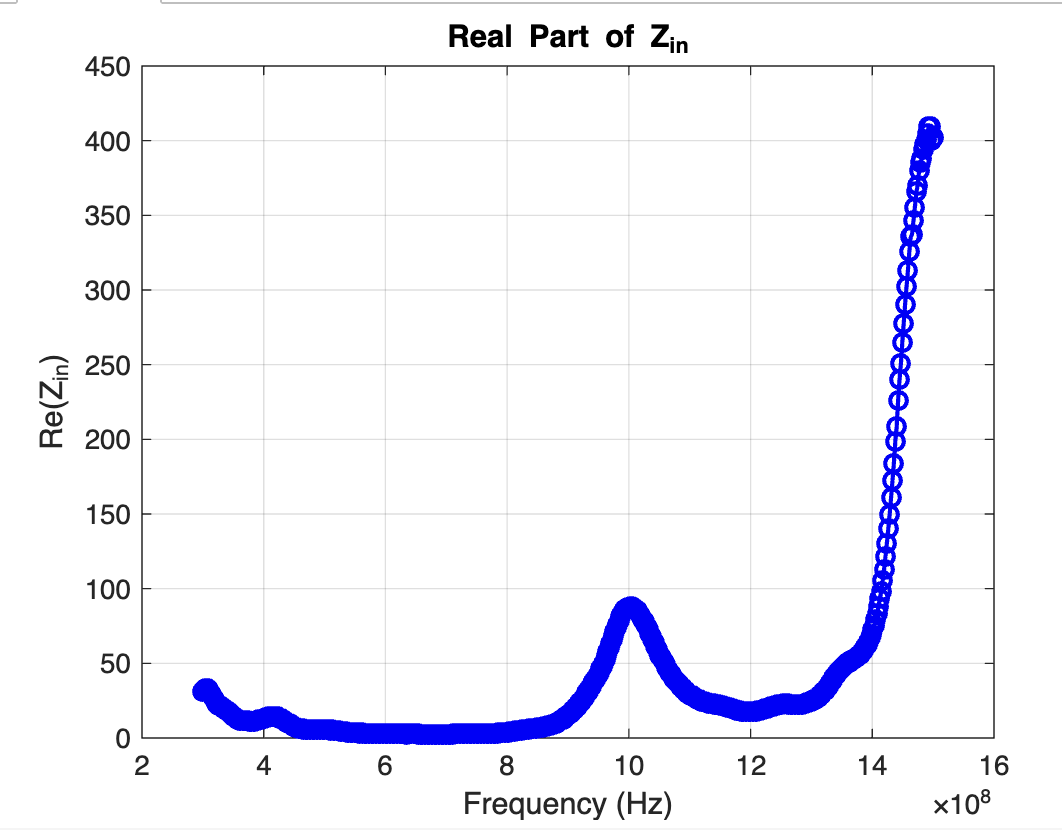
\includegraphics[width=0.5\textwidth]{./image/figure11.png}
              \caption{Real Part of Input Impedance}
          \end{figure}
          \begin{figure}[H]
              \centering
              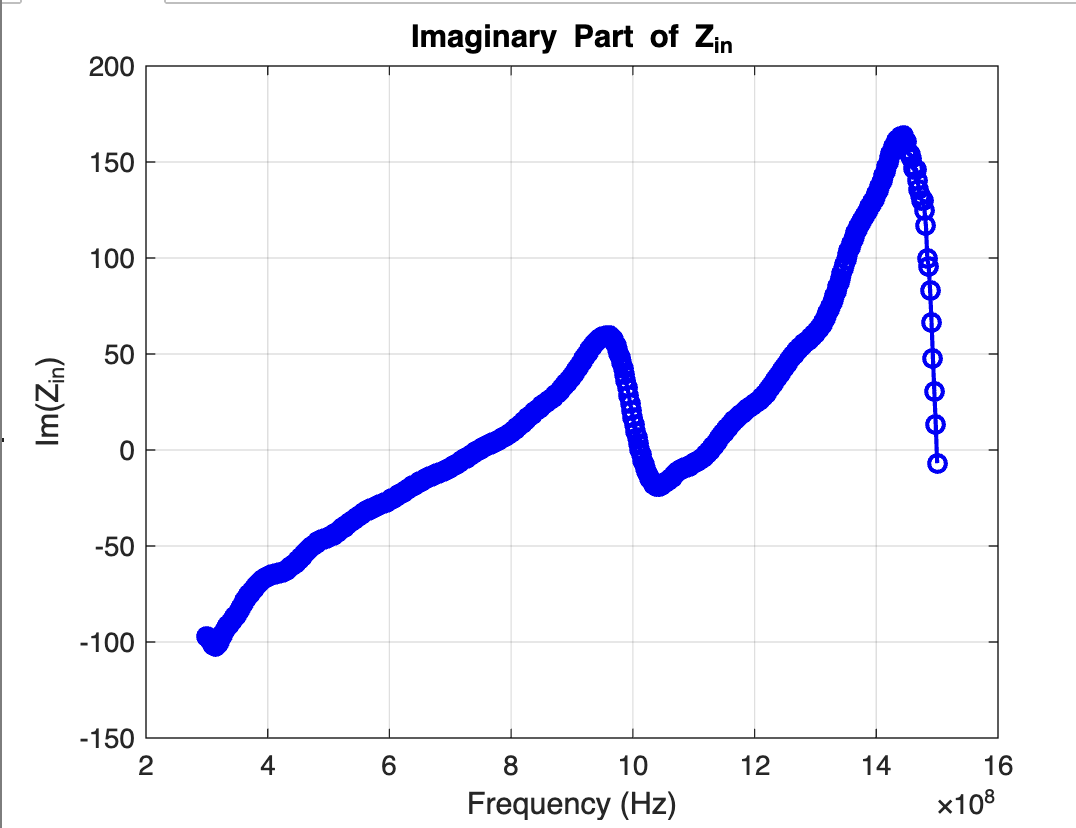
\includegraphics[width=0.5\textwidth]{./image/figure12.png}
              \caption{Imaginary Part of Input Impedance}
          \end{figure}
    \item The radiation pattern roughly corresponds to a $\sin^2 (\theta)$ function, which matches the calculations from the lecture.
          \begin{table}
              \centering
              \begin{tabular}{|c|c|}
                  \hline
                  \textbf{Angle (degrees)} & \textbf{$S_{21}$ (dB)} \\
                  \hline
                  0                        & -47.5568               \\
                  10                       & -43.7025               \\
                  20                       & -43.4709               \\
                  30                       & -37.9321               \\
                  40                       & -38.1531               \\
                  50                       & -37.0680               \\
                  60                       & -35.2296               \\
                  70                       & -35.4238               \\
                  80                       & -34.4441               \\
                  90                       & -35.7184               \\
                  100                      & -36.4169               \\
                  110                      & -38.5529               \\
                  120                      & -39.9543               \\
                  130                      & -42.2198               \\
                  140                      & -45.5597               \\
                  150                      & -47.8392               \\
                  160                      & -51.1367               \\
                  170                      & -49.8512               \\
                  180                      & -44.6069               \\
                  \hline
              \end{tabular}
              \caption{$S_{21}$ when Dipole Antenna Faces Different Angle}
          \end{table}
          \begin{figure}[H]
              \centering
              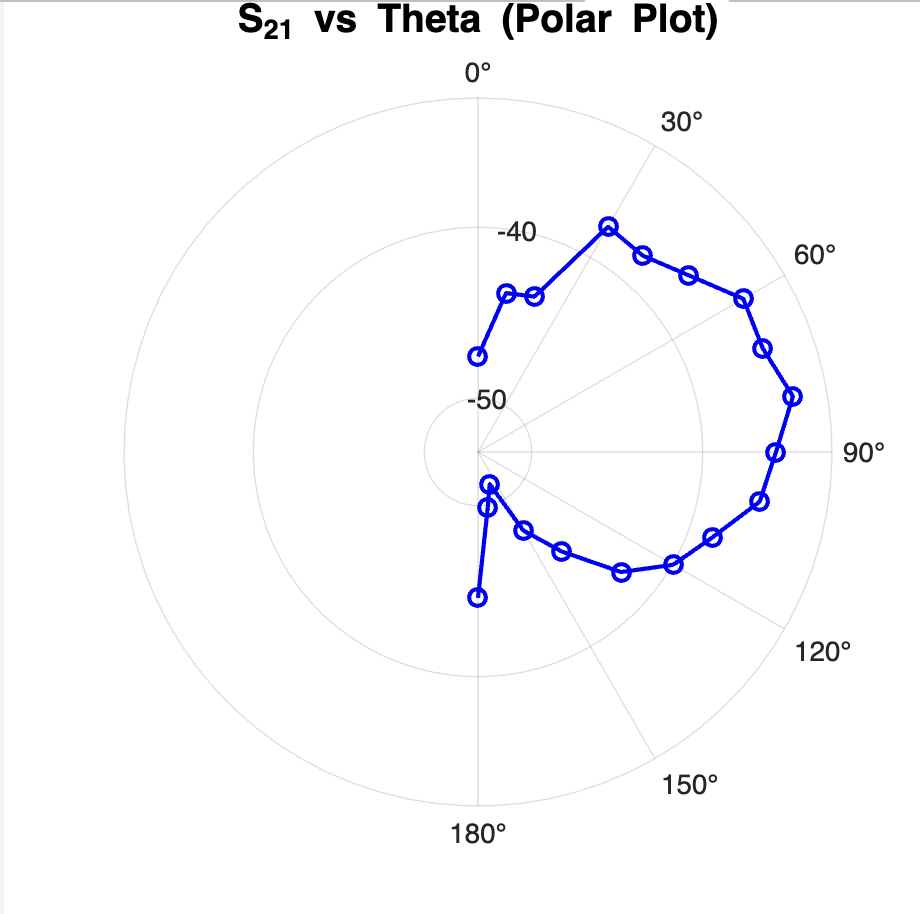
\includegraphics[width=0.5\textwidth]{./image/figure13.png}
              \caption{Polar Plot of S21}
          \end{figure}
    \item The $S_{2,1}$ measured at step 4 is $-33$ dB. Before turning the antenna, we measured that $S_{2,1} = -44.6$ dB. The transmission coefficient increases after we turned the antenna, likely because the field's polarization of the transmitter antenna better matches that of the receiver antenna.
\end{enumerate}



\end{document}
